%!TEX root = main.tex
\setcounter{chapter}{6}
\setcounter{section}{2}
\setcounter{theorem}{0}
\setcounter{equation}{0}

\lectureheader{161}{Calculus I}{Volumes by cylindrical shells}{\textit{Thomas' Calculus} \thesection}

\begin{theorem}[Volume by cylindrical shells]
Let $L\le a<b$, and let $f$ be continuous on $[a,b]$.
The volume of the solid of revolution obtained by rotating the region between the $x$-axis and the graph of $y=f(x)$ from $x=a$ to $x=b$ about the vertical line $x=L$ is
\begin{equation*}
V = 2\pi \int_a^b(x-L)f(x)\dee x.
\end{equation*}
\end{theorem}
\begin{remark}\,
\begin{itemize}
\item We call this formula the method of cylindrical shells.
\item Near $x$, the radius of shell is $x-L$, the height of the shell is $f(x)$, and its thickness is $\dee x$.
\end{itemize}
\end{remark}
\begin{center}
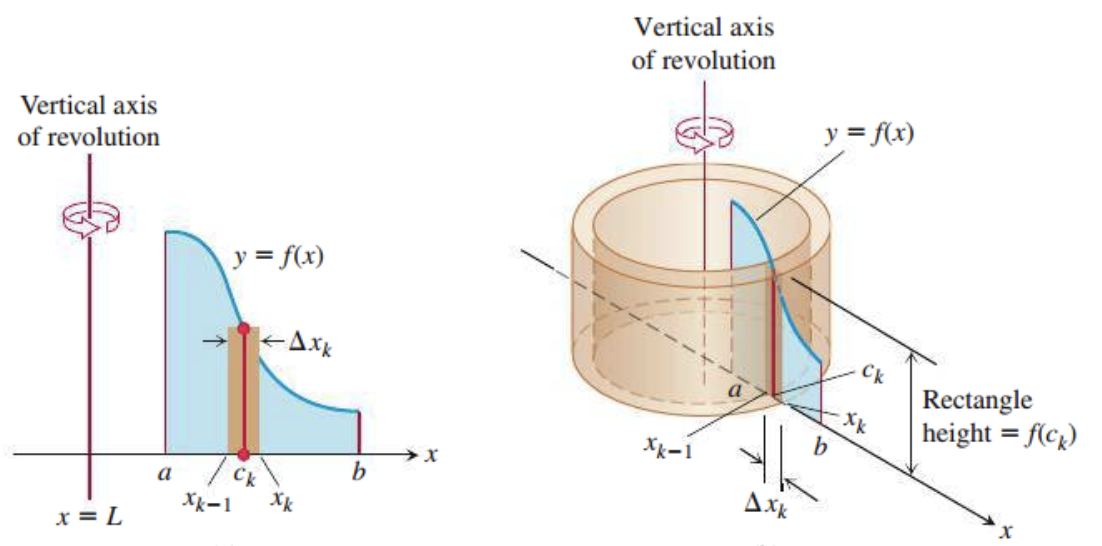
\includegraphics[width=6in]{img/cylindrical_shell}
\end{center}
\begin{remark}\,
\begin{itemize}
\item An analogous formula works when revolving regions about horizontal axes as well.
\item If a 2D region is revolved about an axis to form a solid of revolution, then\dots
\begin{itemize}
\item the method of disks and washers (i.e., cross-sections) involves integrating along the axis of rotation.
\item the method cylindrical shells involves integrating from the axis of rotation to the edge along a perpendicular axis.
\end{itemize}
\item Some volumes can be computed using either method, but it is often the case that one method is preferable.
\end{itemize}
\end{remark}

\newpage

\begin{example}
The region enclosed by the $x$-axis and the parabola $y=f(x)=3x-x^2$ is revolved about the vertical line $x=-1$ to generate a solid.
Find the volume of the solid.
\end{example}

\newpage

\begin{example}
The region bounded by the curve $y=\sqrt x$, the $x$-axis, and the line $x=4$ is revolved about the $y$-axis to generate a solid.
Find the volume of the solid.
\end{example}

\newpage

\begin{example}
The region bounded by the curve $y=\sqrt x$, the $x$-axis, and the line $x=4$ is revolved about the $x$-axis to generate a solid.
Find the volume of the solid.
\end{example}
